\chapter{Trabajo desarrollado}
\thispagestyle{empty}


En este capítulo se explican las funcionalidades básicas del simulador desarrollado centradose únicamente en los aspectos más importantes. Para profundizar más sobre estos aspectos debe acudir a los anexos.

\section{Resumen del simulador}
\thispagestyle{empty}

Se trata de un sistema de colaboración abierta distribuida que permite configurar distintos escenarios con objetos móviles y estáticos sobre mapas de ciudades reales obtenidos a partir del servicio de mapas de OpenStreetMap. 

El simulador de escenarios está basado en el simulador Mavsim desarrollado por el Grupo de Sistemas de Información Distribuidos de la Universidad de Zaragoza utilizado para la simulación de VANETs en el cual hay muchos vehículos distribuidos en una amplia zona geografica.

\begin{figure}[H]
\centering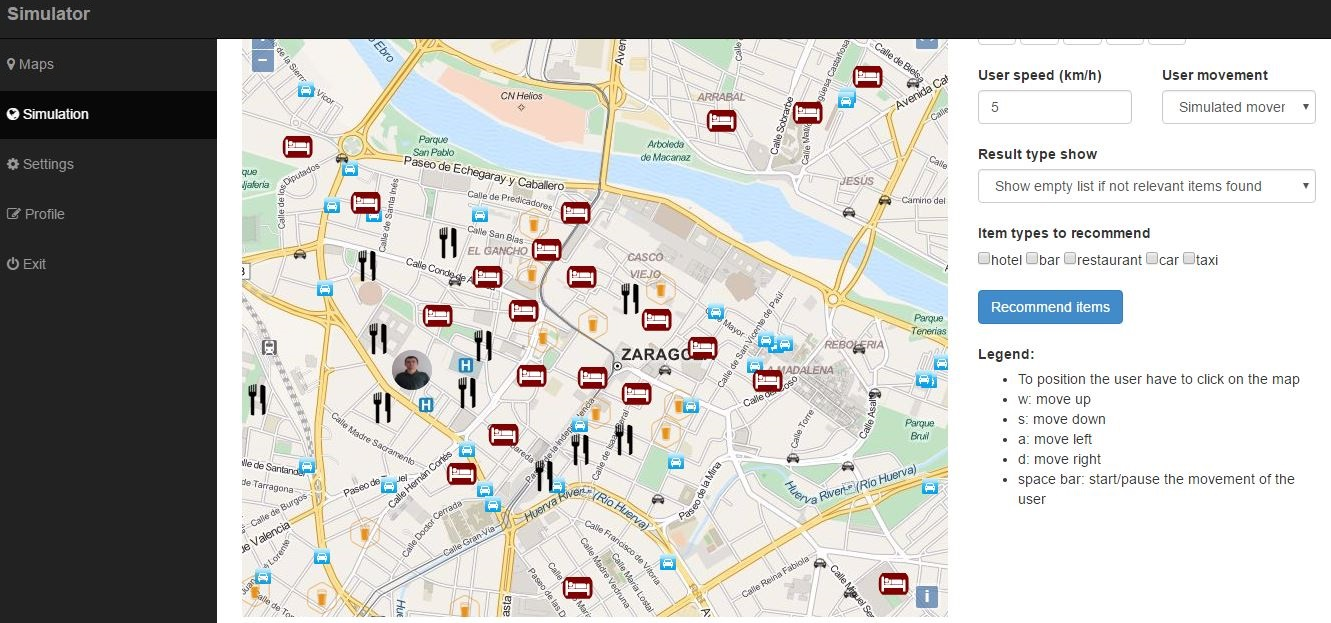
\includegraphics[scale=0.3]{imagenes/resumen-simulador.jpg}
\caption{Simulación en Actur, Zaragoza con un solo usuario}
\label{c2_trama}
\end{figure}

Puede ser usado a través de cualquier dispositovo (PC, tablet, móvil etc.) con conexión a Internet y un navegador web. Permite a los usuarios crear sus propios mapas y escenarios. Durante la creación de una escena el usuario elige cual es la cuidad donde se realiza la simulación, el recomendador a utilizar, si el mapa es colaborativo o no, introducir los objetos estáticos y configurar cuales son los objetos móviles y sus rutas. 

Para realizar una simulación el usuario tiene que buscar y seleccionar el mapa y escenario donde moverse tanto para obtener recomendaciones como para realizar votaciones sobre los distintos objetos de este entorno.

\section{Arquictura del sistema}
\thispagestyle{empty}

La arquitectura del sistema consta de cliente o navegador web, servidor web Node.js, servidor de recomendaciones y base de datos mongoDB (figura \ref{arquitecturaComponentes}).

El la figura \ref{arquitecturaComponentes} observamos que el navegador web se conecta al servidor Node.js mediante dos maneras: la primera es HTTP y la segunda es un sistema bidireccional dirigido por eventos. Las funcionalidades como creación de escenas, busqueda de mapas etc. están desarrollados sobre una REST API y el intercambio de mensajes JSON.

El sistema bidireccional dirigido por eventos es utilizado por una parte durante la simulación, para reflejar los eventos generados por un usuario al resto de usuarios, y por otra para integrar el navegador, el servidor Node.js y el recomendador. De esta manera conseguimos compartir informácion entre los distintos componentes sin que estos los hayan solicitado y evitamos muchas peticiones innecesarias.

\begin{figure}[H]
\centering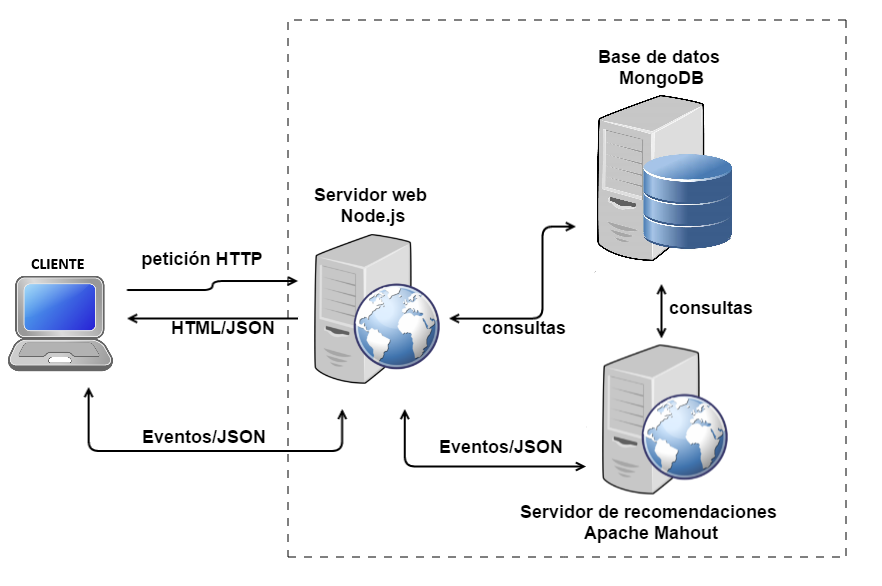
\includegraphics[scale=0.4]{imagenes/arquitectura-componentes.png}
\caption{Arquitectura de componentes del sistema}
\label{arquitecturaComponentes}
\end{figure}

\subsection{Arquitectura del front end}
\thispagestyle{empty}

Para el desarrollo del front end se han utilizado los frameworks Angular.js y bootstrap. Angular.js es un framework que nos permite desarrollar aplicaciones de una sola página. Se ha decidido utilizar esta tecnología porque nos ofrece varias ventajas: ahorro de recursos\footnote{angular.js va transmitiendo las vistas de la interfaz gráfica y las cáchea al lado del cliente para ser reutilizadas posteriormete. Vuelve a solicitar una vista si y solo si esta ha sufrido algún cambio en el servidor} y mejora de la productividad.

Bootstrap es un framework que nos ofrece un sistema de componentes reutilizables y adaptables a la pantalla del dispositivo. De está manera obtenemos una interfaz gráfica que funcione sobre dispositivos móviles. Esto nos da la oportunidad de realizar una simulación sobre un dispositivo móvil y de utilizar la posición geográfica del usuario para obtener recomendaciones en el entorno de una cuidad real. De está manera obtenemos datos reales y muchas más precisión a la hora de evaluar los algoritmos de recomendaciones. 

\begin{figure}[H]
\centering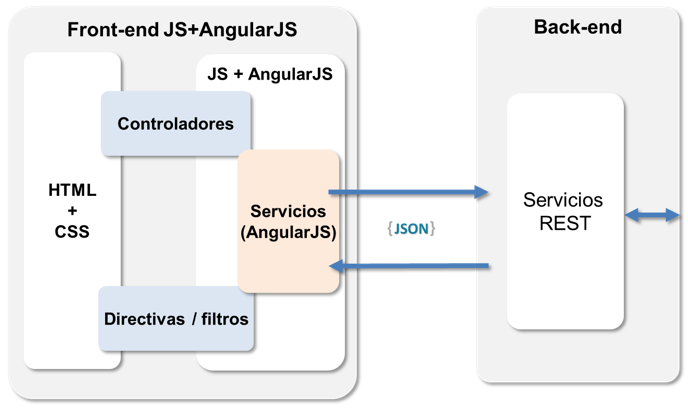
\includegraphics[scale=0.6]{imagenes/arquitectura-front-end.png}
\caption{Arquitectura del front end}
\label{arquitecturaFrontEnd}
\end{figure}

\subsection{Arquitectura del back end}
\thispagestyle{empty}

Poner la arquitectura del back end.

\subsection{Arquitectura de recomendador}
\thispagestyle{empty}

Poner la arquitectura del recomendador

\subsection{Modelo de la base de datos}
\thispagestyle{empty}

Poner el esquema relacional de la base de datos